
\chapter{Introducción}
\label{chap:intro} 
El principal objetivo del proyecto es mejorar la plataforma \textit{Websim} para disponer de más robots y ejercicios para incrementar su valor educativo dando más posibilidades de aprendizaje. 
   
 \section{Tecnologías web}
\label{sec:web}
Las tecnologías web han ido evolucionando a los largo de la historia, pero todas se basan en un modelo cliente-servidor. Para lograr la comunicación entre cliente y servidor, se necesita un navegador por parte del cliente y un servidor web capaz de atender las solicitudes. El protocolo que es utilizado para esta comunicación se llama \textit{HTTP}.
\subsection{HTTP}
\label{subsec:http}

\subsection{Tecnologías en servidor}
\label{subsec:tecserver}

\subsection{Tecnologías en cliente}
\label{subsec:tecclient}


\section{Robótica}
\label{sec:robotica}
La robótica es una rama tecnológica encargada del diseño y construcción de aparatos que realizan operaciones y trabajos en sustitución de la mano de obra humana. 

Un robot es un sistema autónomo programable capaz de realizar tareas de ayuda al ser humano y con aplicaciones en campos diversos como medicina, hogar, fábricas, etc. 

Los robots se componen de sensores, controladores y actuadores.
\begin{itemize}
    \item Sensores: son los encargados de recoger información del entorno. En este grupo se encuentran láser, cámaras, ultrasonidos u odómetros. Estos dispositivos equivalen a los sentidos humanos. 
    \item Controladores: analizan los datos recogidos por los sensores y elaboran una respuesta que va a ser enviada a los actuadores. En los seres humanos equivale al cerebro. 
    \item Actuadores: se encargan de transformar energía eléctrica, hidráulica o neumática en mecánica. Son los interactúan con el entorno y equivalen a los músculos humanos. 
\end{itemize}

\subsection{Historia}
La palabra robot fue empleada por primera vez en 1920 por Karel Capek, un escritor checo que realiza una obra de teatro en la que un hombre fabrica un robot. 

Años más tarde, en 1950, Isaac Asimov publica un libro llamado \textit{Yo, Robot} en el que acuña la palabra robótica definiendo a la ciencia que estudia a los robots. En el también se incluyen tres leyes de la robótica:
\begin{itemize}
    \item Un robot no hará daño a un ser humano ni permitirá que un ser humano sufra ningún tipo daño.
    \item Un robot debe cumplir las órdenes recibidas por un ser humano, salvo las que entren en conflicto con la primera ley.
    \item Un robot debe proteger su propia existencia mientras que no entre en conflicto con ninguna de las leyes anteriores. 
\end{itemize}{}

Es a finales de la década de los 50 cuando la robótica sufre el mayor impulso al crearse el primer robot comercial en 1956 y, años más tarde, en 1961, se instala el primer robot industrial (Figura \ref{fig:unimate}).  

\begin{figure}[H]
\centering
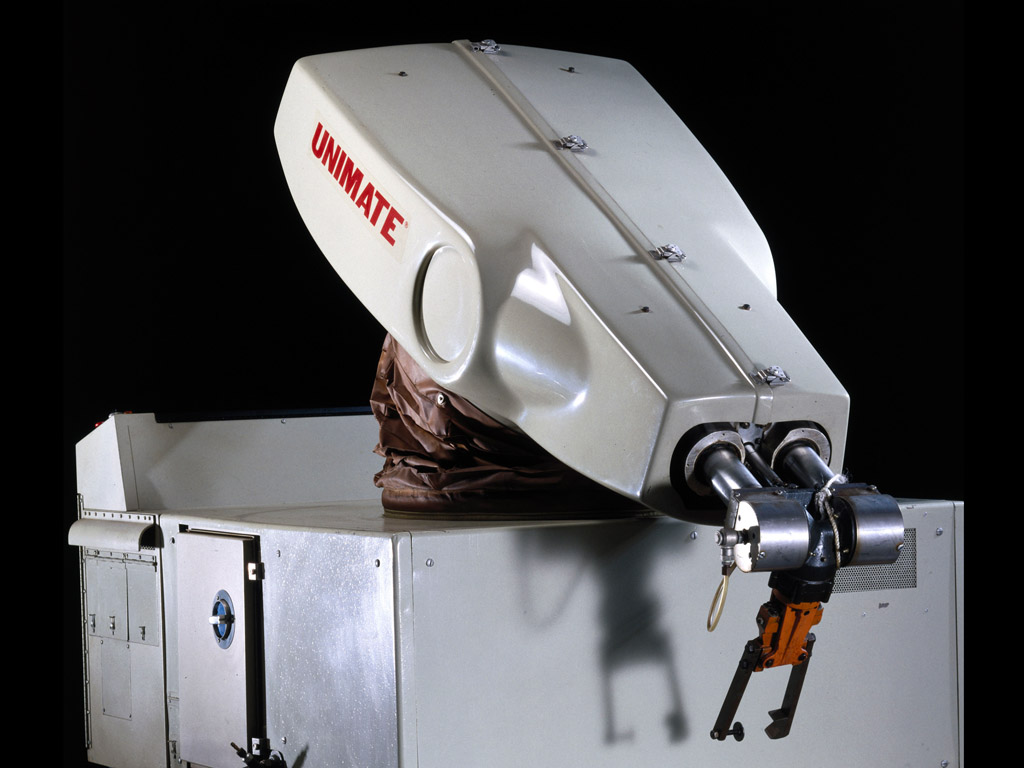
\includegraphics[scale=0.2]{img/unimate.jpg}
\caption{Unimate, primer robot industrial} \label{fig:unimate}
\end{figure}

En los años 70 se crea el primer robot autónomo, \textit{Shakey}  (Figura \ref{fig:shakey}). Fue el primero que incorporaba inteligencia artificial y disponía de control de motores y sensores. \textit{Shakey} era capaz de recoger toda la información de su entorno, crear un mapa y diseñar el camino más corto desde su ubicación al destino. 


\begin{figure}[H]
\centering
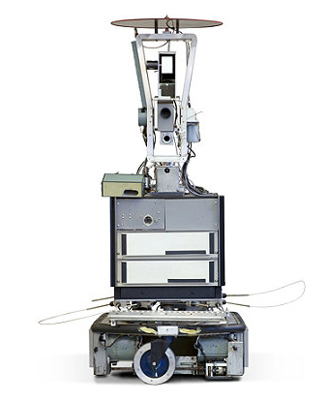
\includegraphics[width=0.5\textwidth]{img/shakey.jpg}
\caption{Shakey, primer robot autónomo} \label{fig:shakey}
\end{figure}

En 2000 la compañía Honda lanza el robot \textit{Asimo} (Figura \ref{fig:asimo}), un robot humanoide capaz de detectar múltiples objetos, reconocer caras e interpretar comandos de voz o gestos.\textit{Asimo} fue creado con el objetivo de, algún día, ofrecer asistencia a personas con necesidades especiales. 

\begin{figure}[H]
\centering
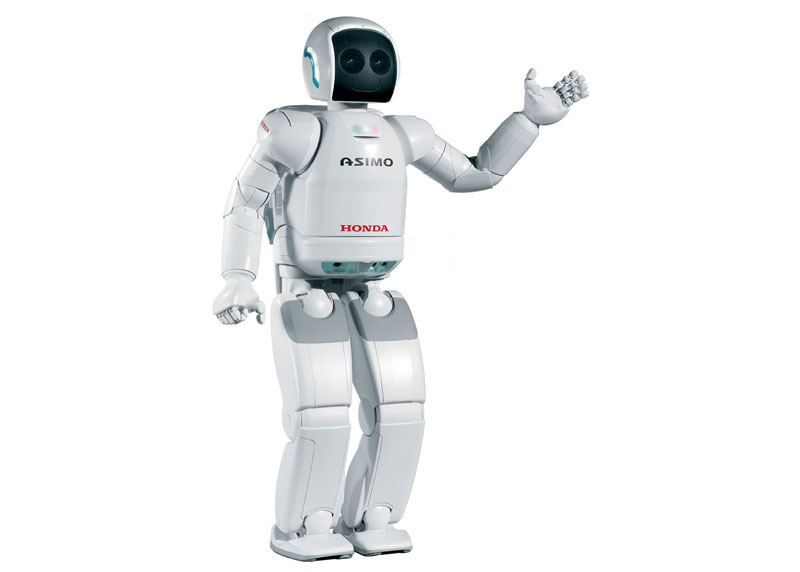
\includegraphics[width=0.5\textwidth]{img/asimo-honda.jpg}
\caption{Asimo, primer robot humanoide} \label{fig:asimo}
\end{figure}

Es en 2011 cuando la robótica alcanza uno de sus mayores hitos gracias al robot explorador \textit{Curiosity} (Figura \ref{fig:curiosity}). Este robot llego a Marte en 2012 y su cometido fue investigar el planeta para determinar si existió vida en Marte, caracterizar su clima y geología y preparar el entorno para su exploración humana. 

\begin{figure}[H]
\centering
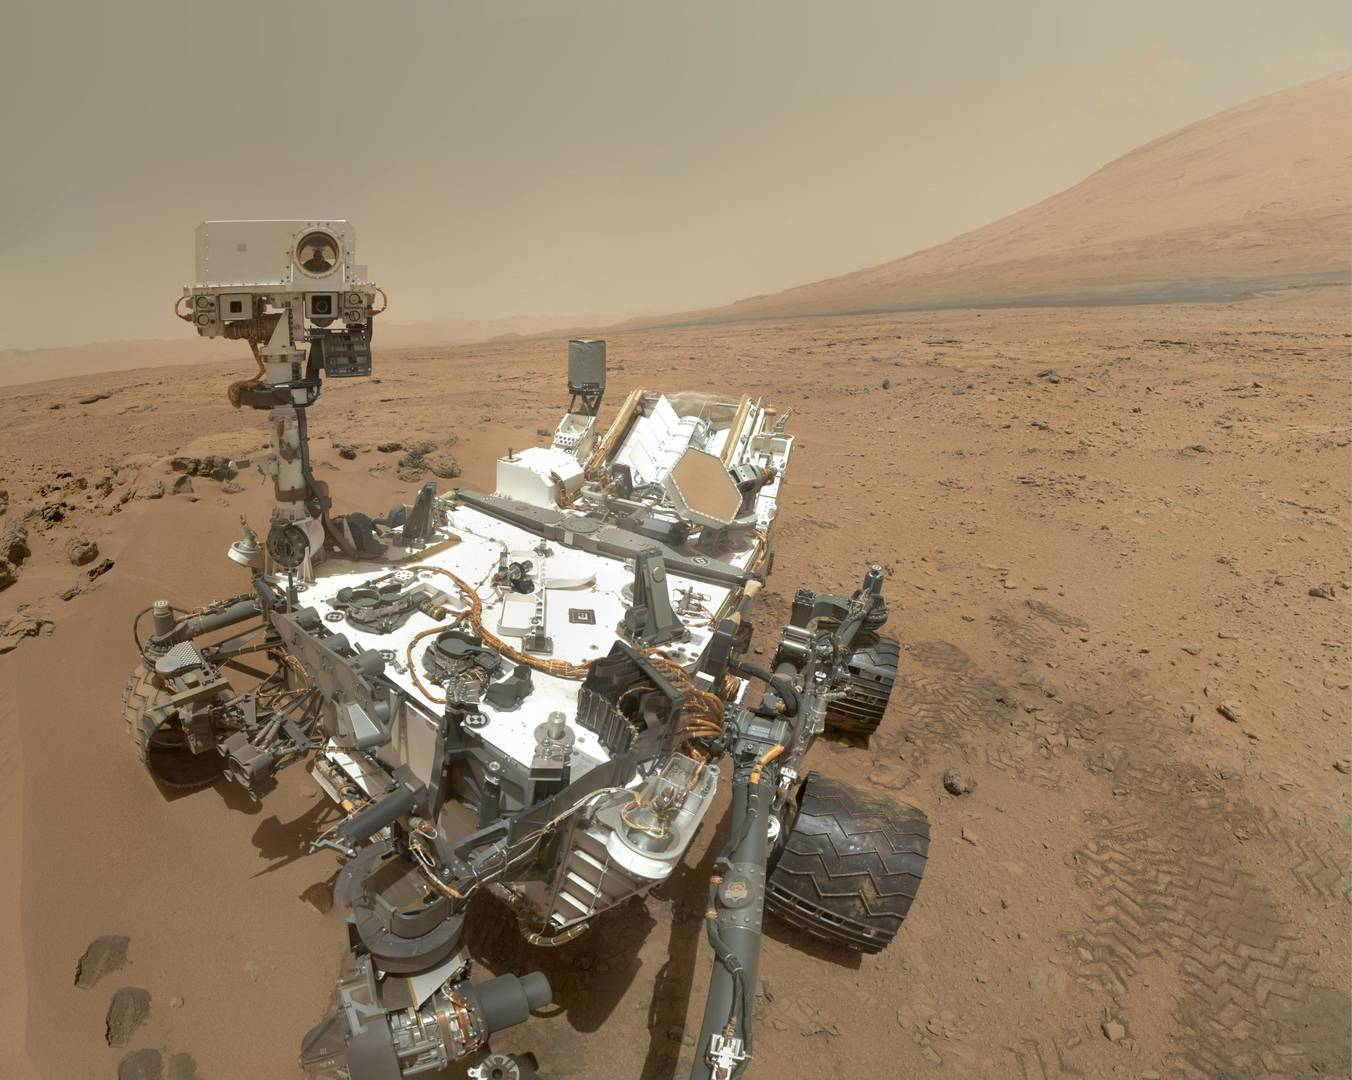
\includegraphics[width=0.8\textwidth]{img/curiosity.jpg}
\caption{Autorretrato del Curiosity en Marte} \label{fig:curiosity}
\end{figure}


Hoy en día no solo se ven robots en entornos industriales, si no que aparecen cada vez más en entornos domésticos, educativos o automovilístico.

\subsection{Tipos de robots}
\label{subsec:tiposRobots}


\section{Robótica educativa}
\label{sec:educativa}

\chapter{Objetivos}
\label{chap:objetives}
\section{Objetivos}
\section{Metodología}
